%\section*{Methods}
\section*{\textbf{\underline{Methods}}}
\subsection*{\textbf{Random field strength}}
In the methods we explain that a random gaussian field with a random strength was added into each landscape we modelled so that each virtual species occurs in a unique species. In Figure \ref{fig:S1} we show how different levels of strength in the random field can lead to different levels of spatial autocorrelation in the environmental variable across the landscape.

\begin{figure}[h!]
\centering
%\graphicspath{ {c:/Teste/Chapter-1-Protocol/Manuscript/Plots/} }
\centerline{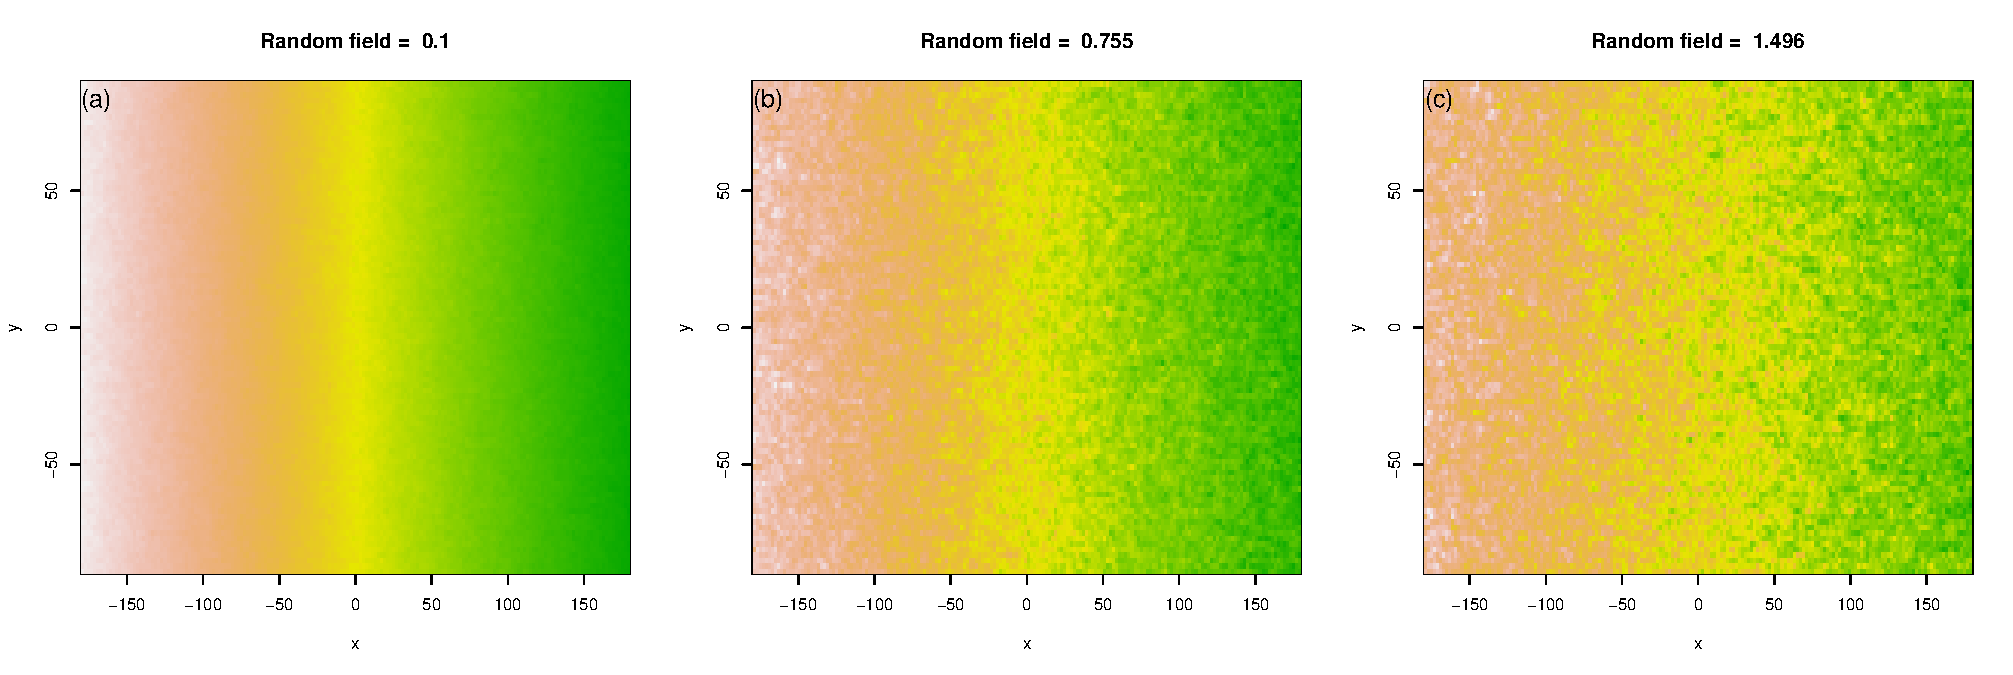
\includegraphics[width=1\textwidth]{Plots/FigureS1}}
\caption[Random fields]{Effects of the strenght of the random field on the virtual environmental gradient. As the strength of the random field increases from 0.1 (a), to 0.755 (b) and 1.49 (c) the landscape becomes less spatially autocorrelated.}
 \label{fig:S1}
\end{figure}

\subsection*{\textbf{Using unique occurrence points for model cross-validation}}
In the methods we mentioned that for the virtual species we modelled their distribution using a unique set of occurrence points for each of the 20 sampling process applied during the cross-validation of the models. To ensure that this process is comparable to the one applied to the real species (i.e., the same occurrence points were resampled 20 times), we also resampled the same set of occurrence points for 20 virtual species modelled their distribution and compared whether the performance and variation in performance of these models greatly differ from each other. In general, we found that both the model performance and variation in performance are very similar when the same and unique data are used to model the species distributions (Figure \ref{fig:S2}). This shows that the same results are obtained when both types of data are used in SDMs and that this could not have affected our study.

\begin{figure}[h!]
\centering
%\graphicspath{ {c:/Teste/Chapter-1-Protocol/Manuscript/Plots/} }
\centerline{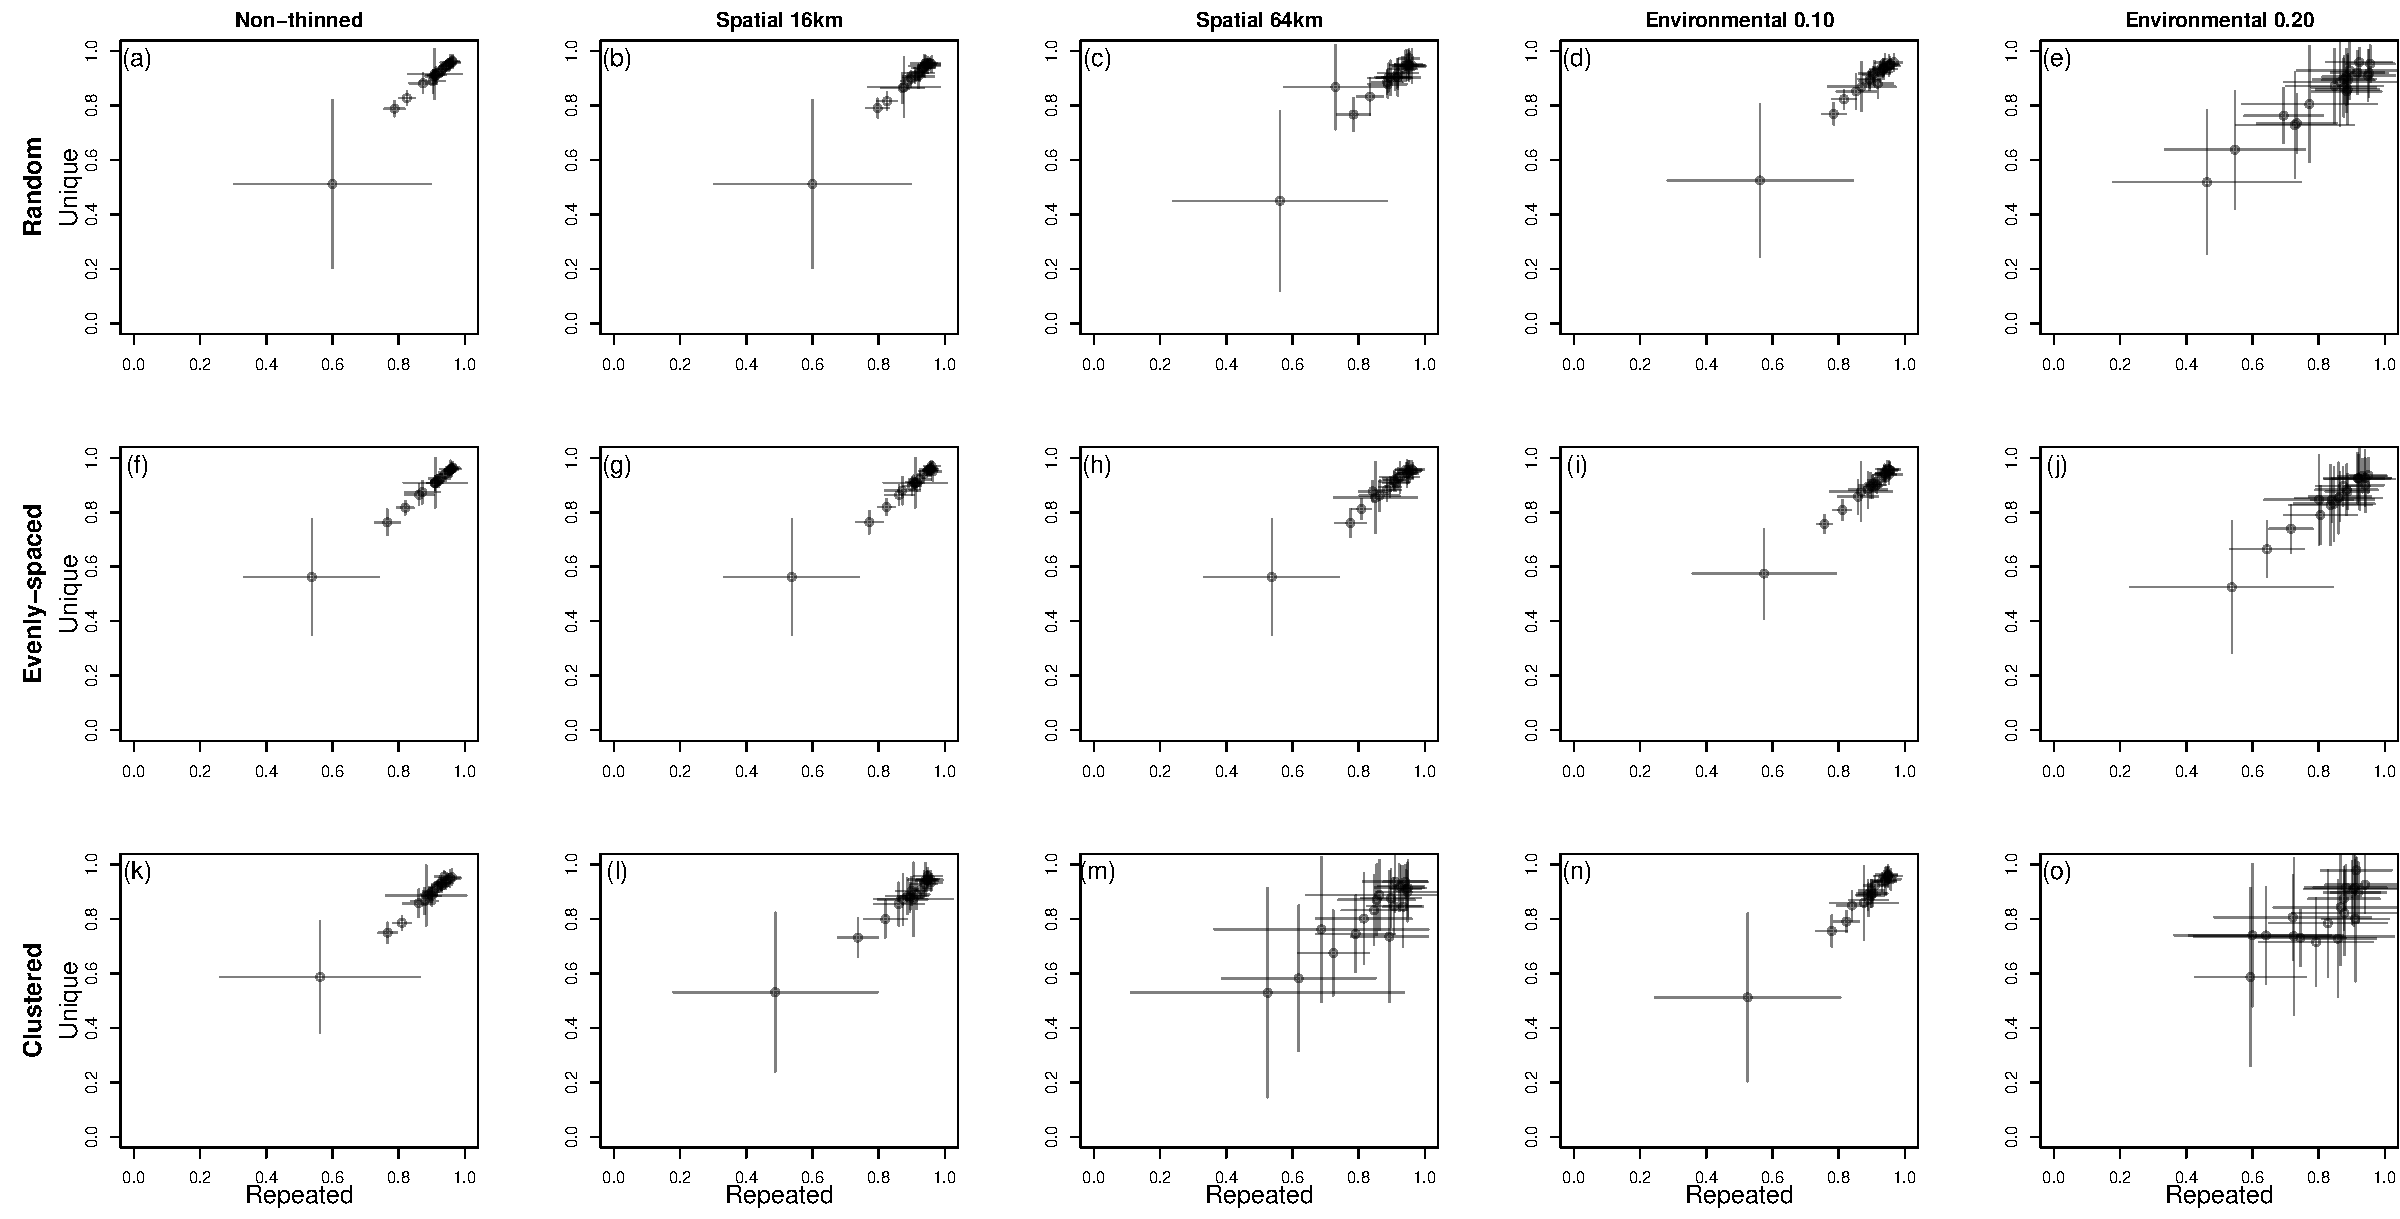
\includegraphics[width=1\textwidth]{Plots/FigureS2}}
\caption[Occurrence data type and model performance]{SDMs discrimination (AUC) when the same (x-axis) and unique (y-axis) data are used in the cross-validation sampling process for 20 virtual species with random (a-e), overdispersed (f-j), and clustered occurrence points (k-o).}
\label{fig:S2}
\end{figure}

\subsection*{\textbf{Estimating root mean square error}}
In the methods we explain that we used root mean square error to measure calibration, a for of model performance, for 10 probability bins (where they have similar sample sizes based on quantiles). We use the formula  $\sqrt{\frac{\Sigma_{i=1}^{n} (x_i - \bar {y})^2}{n}}$ to calculate RMSE for each individual bin, where $x_i$ represents the predicted occurrence probability for a specific cell within a probability bin by a model and $\bar {y}$ is the mean of a binary vector that is equivalent to the fraction of observed occurrences in that probability bin. We used $\bar {y}$ instead of $y_i$ because we only have binary (i.e., 0 and 1) data for the observed occurrences, and using them would affect the estimation of calibration. We averaged calibration across the 10 probability bins for each species considered in our study. 

The advantage of using bins to estimate calibration is that it allows for the consideration of differences in the ability of a model to perform well under different scenarios. For example, we calculated RMSE for a well (i.e., good) and a poorly (i.e., bad) calibrated model, where the predicted suitability in a bin is similar to the observed fraction of occurrences in that bin in a good model but not in the bad model. The good model had a similarly high performance across the different probability bins and, while the bad model had a general lower performance, its performance was even worse for some bins (i.e., the bins with really low or high suitability) than for others (Figure \ref{fig:rmse}). By binning the data we are able to take these differences in the performance of a model into consideration and we provide a more realistic estimation of calibration for the model. 

\begin{figure}[h!]
\centering
%\graphicspath{ {c:/Teste/Chapter-1-Protocol/Manuscript/Plots/} }
\centerline{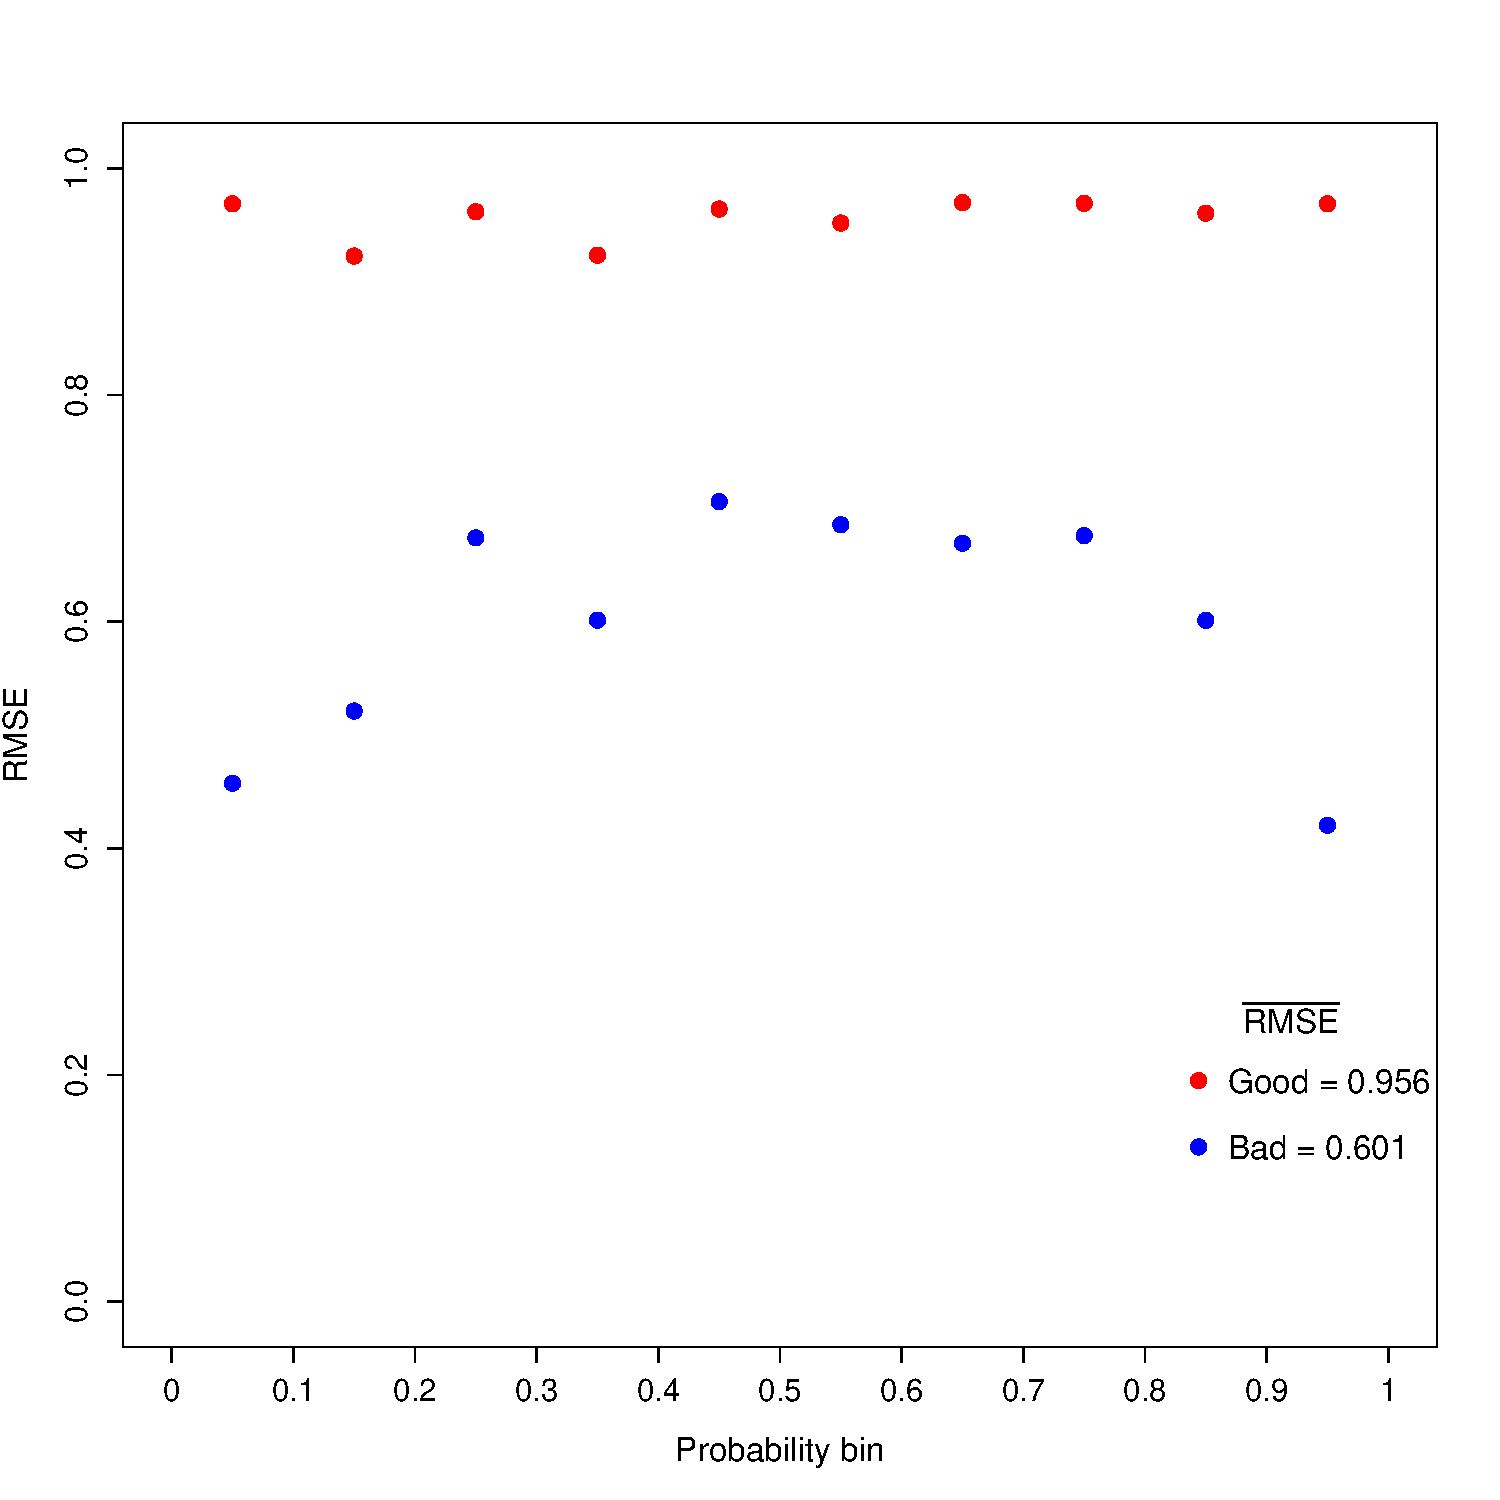
\includegraphics[width=1\textwidth]{Plots/RMSE_bins}}
\caption[Root mean square error]{Calculation of root mean square error (RMSE) for 10 probability bins (i.e., dots in the plot) considering a good and a bad model.}
 \label{fig:rmse}
\end{figure}



%\section*{Results}
\section*{\textbf{\underline{Results}}}


As expected, we found a positive relationship between thinning distance used and number of occurrence points left available for the modeling procedure, such that the amount of occurrence points available to model the species distributions rapidly decline when larger thinning distances are used.  
%\addtocontents{lof}{\protect\vskip-12pt}

\begin{figure}[h!]
\centering
%\graphicspath{ {c:/Teste/Chapter-1-Protocol/Manuscript/Plots/} }
\centerline{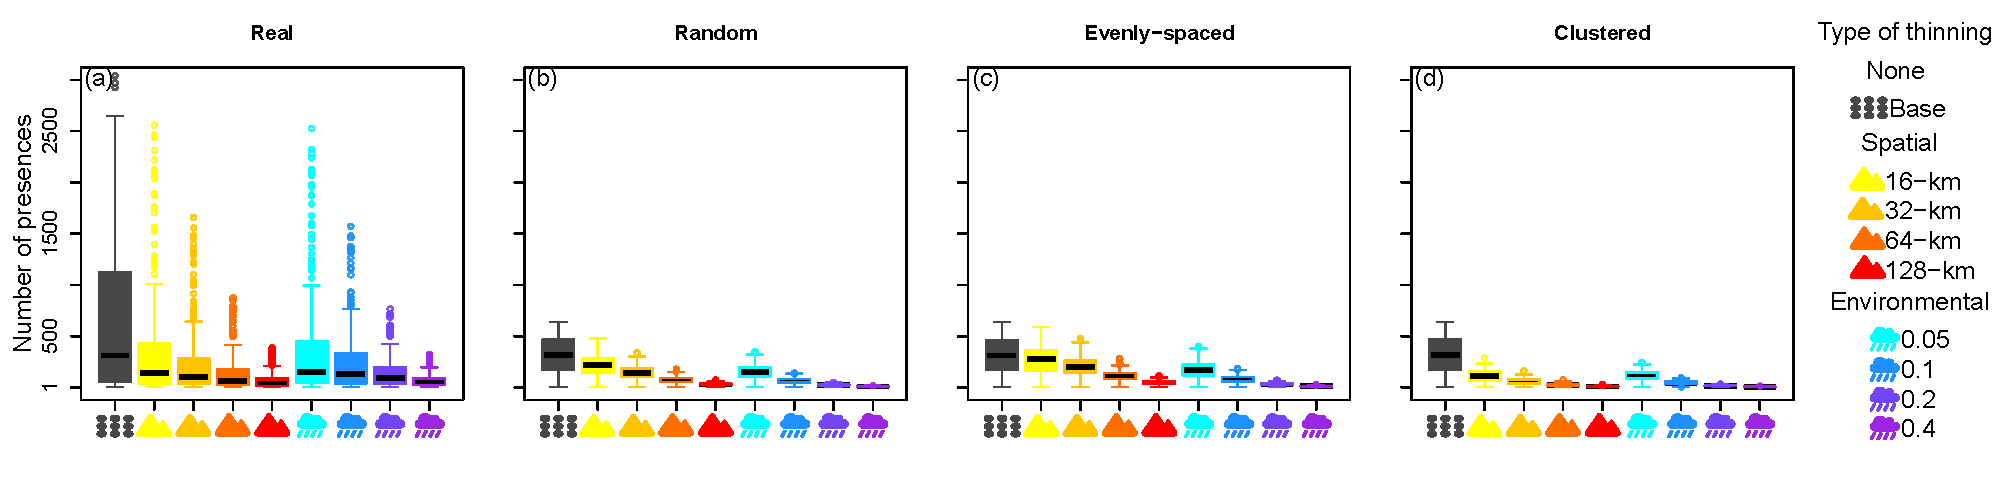
\includegraphics[width=1\textwidth]{Plots/FigureS3}}
\caption[Number of occurrence points]{Number of occurrence points available for the modeling of the real (a), and virtual species with random (b), clustered (c) and evenly-spaced (d) bias}
\label{fig:S3}
\end{figure}

In the results section of the main text we mainly report the effects of thinning occurrence points on the discrimination power of MaxEnt while the effects of thinning on SVM, GLM, and GAM were only briefly mentioned. Here, we describe in details the effects of thinning on the different performance metrics of these modeling methods. 

\subsection*{\textbf{Using MaxEnt}}
%\addtocontents{lof}{\protect\vskip-12pt}

Spatial and environmental thinning decreased MaxEnt accuracy and calibration in a similar manner for real (Figure \ref{fig:S4}a, Figure \ref{fig:S6}a) and virtual (Figure \ref{fig:S4}b-d, Figure \ref{fig:S6}b-d) species. In these cases, spatial thinning had stronger negative effects on MaxEnt accuracy and calibration of real species and virtual species with clustered occurrence points whereas virtual species with random and evenly-spaced occurrence points were more negatively affected by environmental thinning. Nevertheless, the negative effects of environmental thinning on MaxEnt accuracy and calibration were significant and consistent across real and virtual species. Similarly, spatial and environmental thinning also decreased MaxEnt precision of virtual (Figure \ref{fig:S5}b-d) species, where all the species were similarly affected by the thinning approaches, and to a lower degree for real (Figure \ref{fig:S5}a) species. In general, the negative effects of thinning were similar across the different types of spatial biases and tended to be stronger when larger thinning distances were used.

%\addtocontents{lof}{\protect\vskip-12pt}

\begin{figure}[h!]
\centering
%\graphicspath{ {c:/Teste/Chapter-1-Protocol/Manuscript/Plots/} }
\centerline{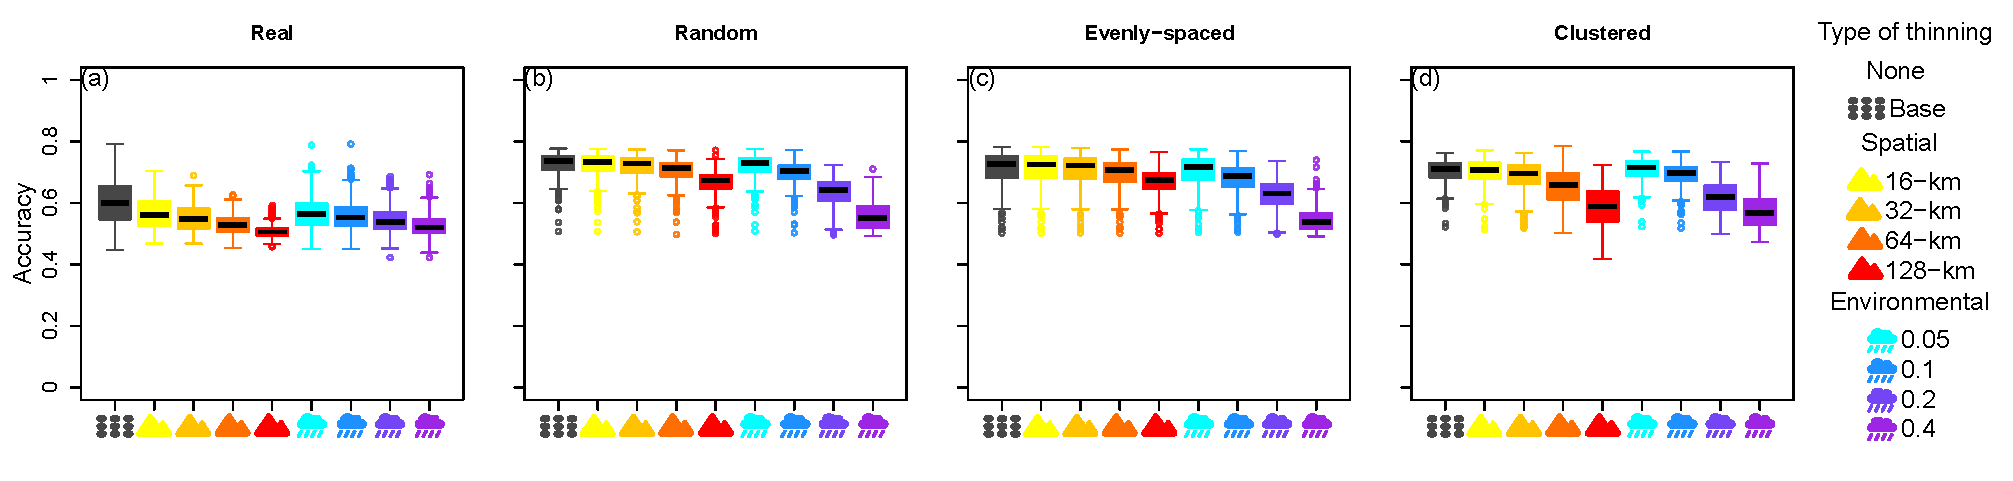
\includegraphics[width=1\textwidth]{Plots/FigureS4}}
\caption[Effects of thinning on MaxEnt accuracy]{The effects of spatial and environmental thinning on MaxEnt accuracy of real species (a), and virtual species with random (b), clustered (c), and evenly-spaced (d) sampled occurrence points.}
 \label{fig:S4}
\end{figure}

%\addtocontents{lof}{\protect\vskip-12pt}

\begin{figure}[h!]
\centering
%\graphicspath{ {c:/Teste/Chapter-1-Protocol/Manuscript/Plots/} }
\centerline{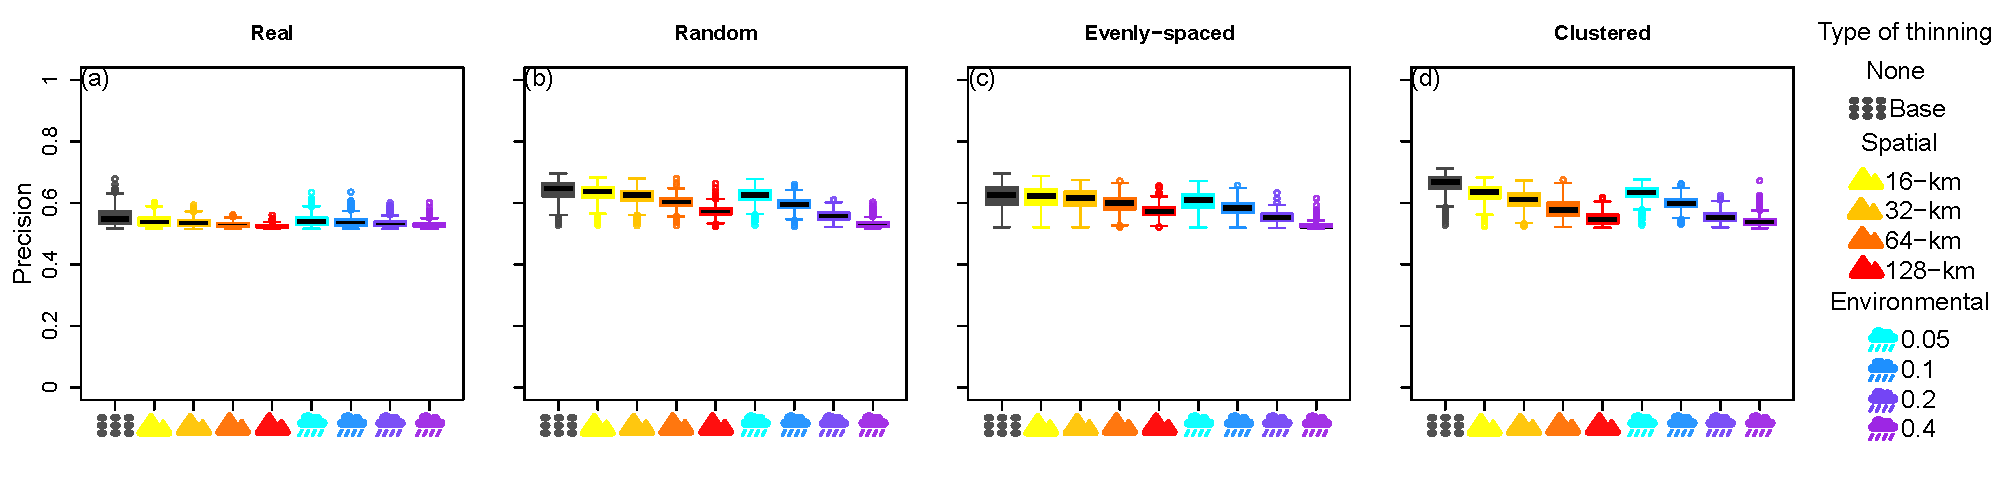
\includegraphics[width=1\textwidth]{Plots/FigureS5}} 
\caption[Effects of thinning on MaxEnt precision]{The effects of spatial and environmental thinning on MaxEnt precision of real species (a), and virtual species with random (b), clustered (c), and evenly-spaced (d) sampled occurrence points.}
 \label{fig:S5}
\end{figure}

%\addtocontents{lof}{\protect\vskip-12pt}

\begin{figure}[h!]
\centering
%\graphicspath{ {c:/Teste/Chapter-1-Protocol/Manuscript/Plots/} }
\centerline{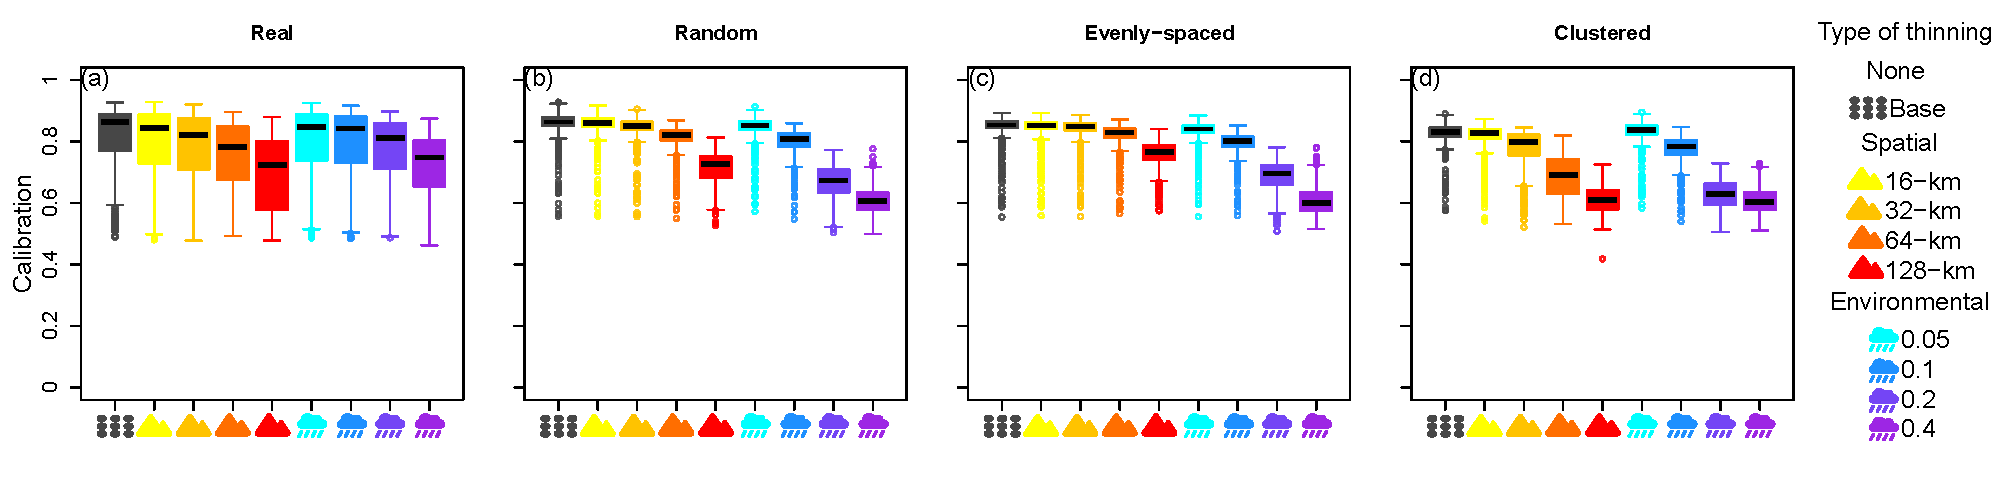
\includegraphics[width=1\textwidth]{Plots/FigureS6}}
\caption[Effects of thinning on MaxEnt calibration]{The effects of spatial and environmental thinning on MaxEnt calibration of real species (a), and virtual species with random (b), clustered (c), and evenly-spaced (d) sampled occurrence points.}
 \label{fig:S6}
\end{figure}

\subsection*{\textbf{Using SVM}}
In general, SVM was less susceptible to the negative effects of thinning occurrence points than GAM and MaxEnt. Spatial and environmental thinning similarly decreased SVM discrimination for real species (Figure \ref{fig:S7}a). On the other hand, only when the largest thinning distances were used did environmental thinning decrease discrimination for virtual species (Figure \ref{fig:S7}b-d). Spatial and environmental thinning decreased SVM accuracy and calibration similarly for real (Figure \ref{fig:S8}a, Figure \ref{fig:S10}a) and virtual species (Figure \ref{fig:S8}b-d, Figure \ref{fig:S10}b-d), where spatial thinning had stronger negative effects on real species and virtual species with clustered occurrences and environmental thinning had stronger negative effects on virtual species with random and evenly-dispersed occurrences. On the other hand, spatial and environmental thinning had only a slight negative effect on SVM precision for real (Figure \ref{fig:S9}a) and virtual (Figure \ref{fig:S9}b-d) species that was observed mostly when the largest thinning distances were used. Thus, although to a lower degree, we still observed a consistent negative effect of thinning on SVM performance across the different types of spatial bias we considered, and these negative effects tended to be stronger the larger the thinning distance used. 




%SVM was the modelling method that was the most resistent to thinning, but the negative impacts were still noticeable especially when larger thinnning distances were used.
\begin{figure}[h!]
\centering
%\graphicspath{ {c:/Teste/Chapter-1-Protocol/Manuscript/Plots/} }
\centerline{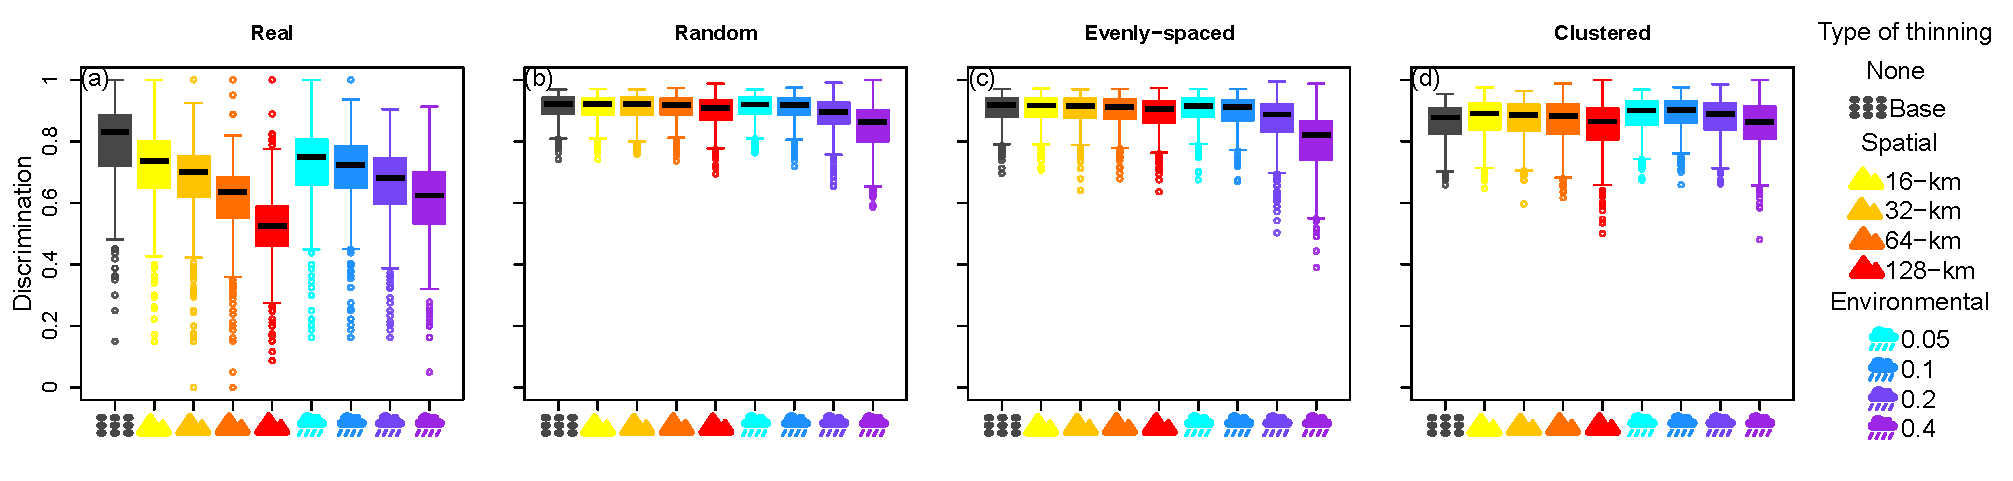
\includegraphics[width=1\textwidth]{Plots/FigureS7}}
\caption[Effects of thinning on SVM discrimination]{The effects of spatial and environmental thinning on SVM discrimination (AUC) of real species (a), and virtual species with random (b), clustered (c), and evenly-spaced (d) sampled occurrence points.}
 \label{fig:S7}
\end{figure}


\begin{figure}[h!]
\centering
%\graphicspath{ {c:/Teste/Chapter-1-Protocol/Manuscript/Plots/}  }
\centerline{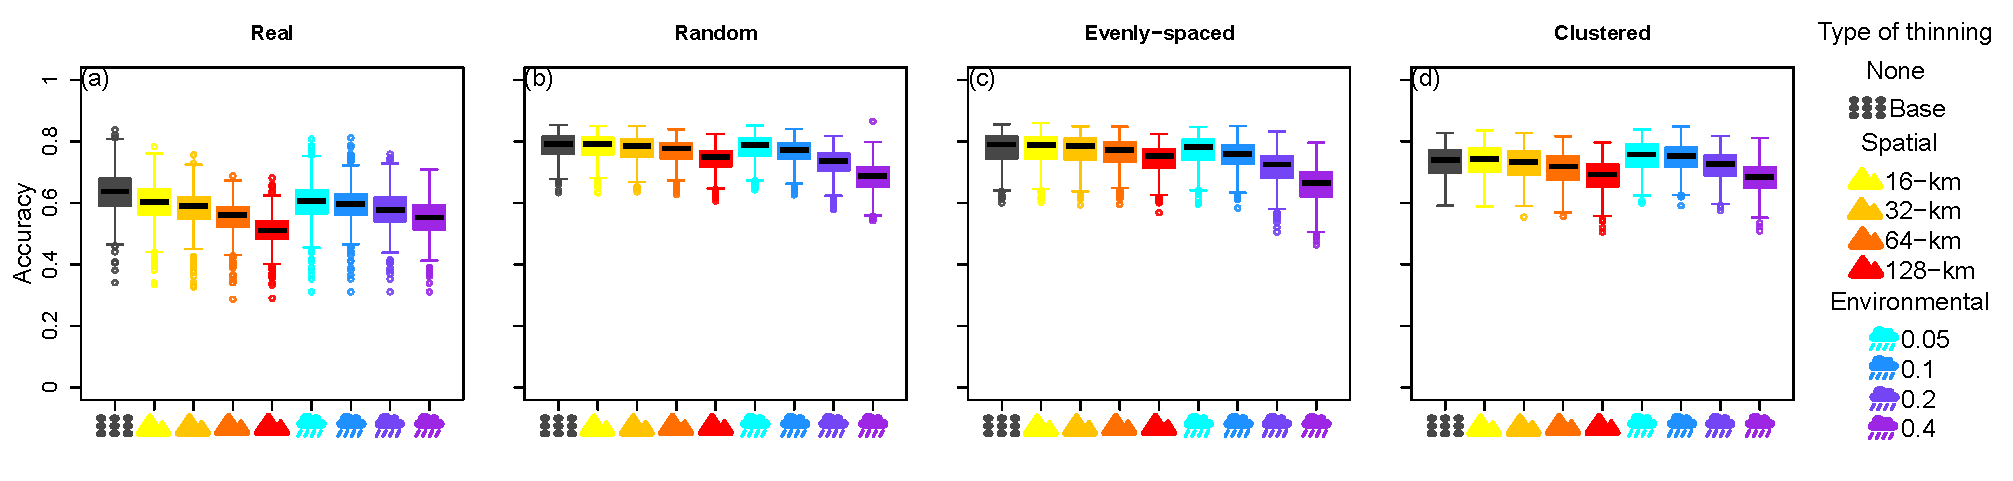
\includegraphics[width=1\textwidth]{Plots/FigureS8}} 
\caption[Effects of thinning on SVM accuracy]{The effects of spatial and environmental thinning on SVM accuracy of real species (a), and virtual species with random (b), clustered (c), and evenly-spaced (d) sampled occurrence points.}
 \label{fig:S8}
\end{figure}

\begin{figure}[h!]
\centering
%\graphicspath{ {c:/Teste/Chapter-1-Protocol/Manuscript/Plots/} }
\centerline{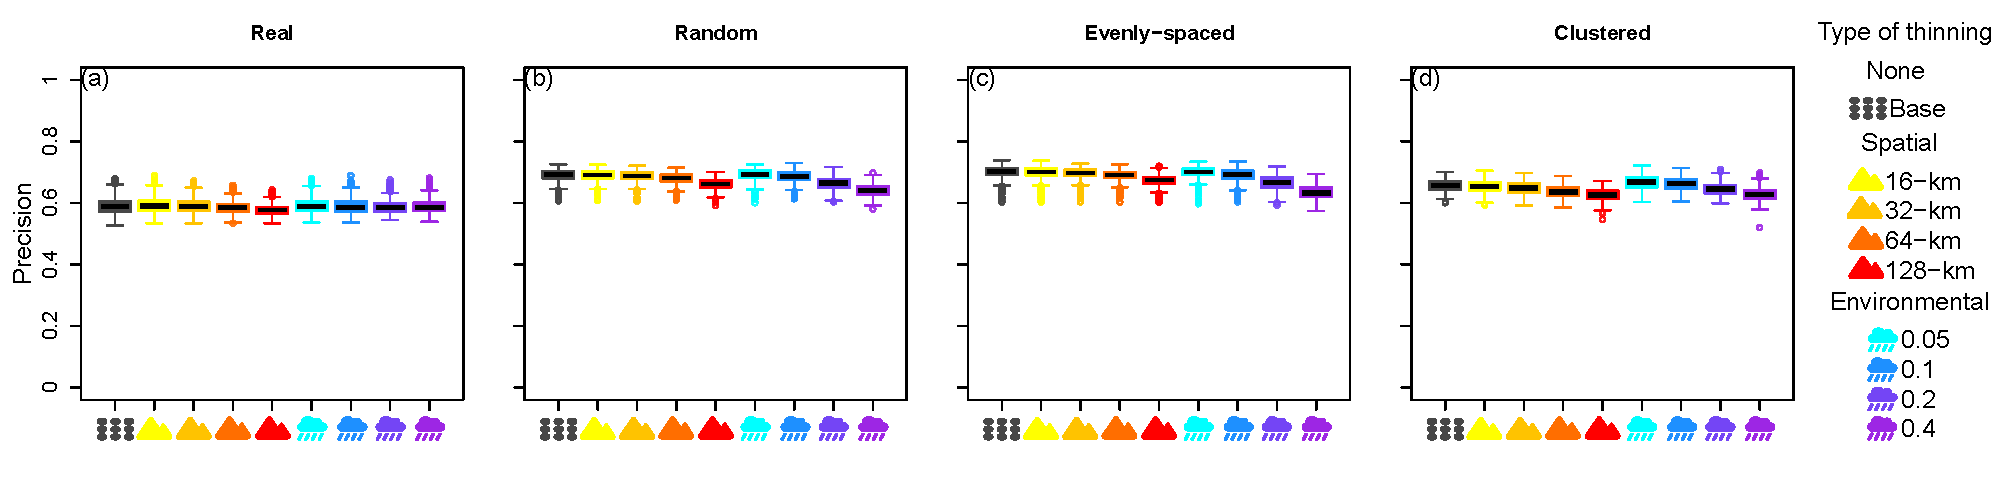
\includegraphics[width=1\textwidth]{Plots/FigureS9}} 
\caption[Effects of thinning on SVM precision]{The effects of spatial and environmental thinning on SVM precision of real species (a), and virtual species with random (b), clustered (c), and evenly-spaced (d) sampled occurrence points.}
 \label{fig:S9}
\end{figure}

\begin{figure}[h!]
\centering
%\graphicspath{ {c:/Teste/Chapter-1-Protocol/Manuscript/Plots/}  }
\centerline{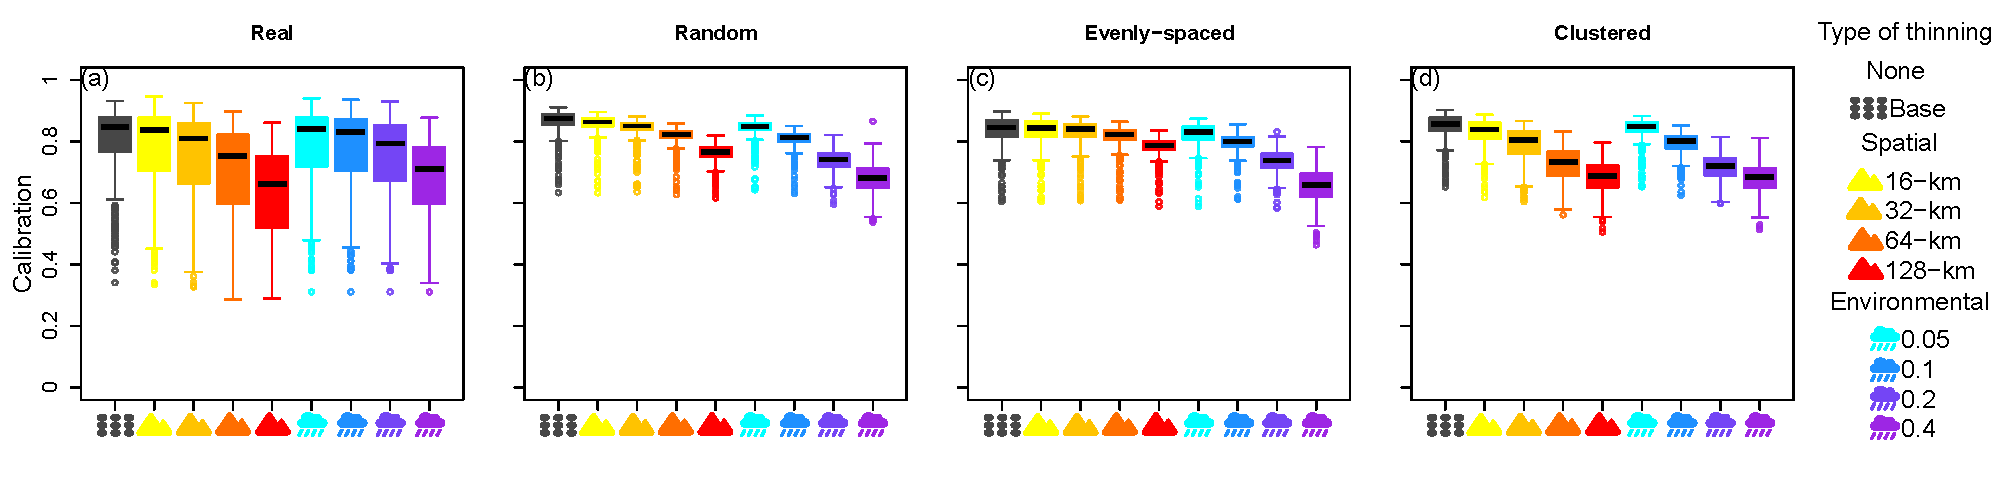
\includegraphics[width=1\textwidth]{Plots/FigureS10}} 
\caption[Effects of thinning on SVM calibration]{The effects of spatial and environmental thinning on SVM calibration of real species (a), and virtual species with random (b), clustered (c), and evenly-spaced (d) sampled occurrence points.}
 \label{fig:S10}
\end{figure}



\subsection*{\textbf{Using GLM}}
Similarly to SVM, thinning also affected GLM performance to a smaller extent. Spatial and environmental thinning decreased discrimination of GLM for real (Figure \ref{fig:S11}a) and virtual (Figure \ref{fig:S11}b-d) species, although the negative thinning effects on virtual species were much smaller and only noticeable when the largest thinning distances were used. While spatial and environmental thinning decreased GLM accuracy for real species (Figure \ref{fig:S12}a), virtual species remained largely unaffected by thinning (Figure \ref{fig:S12}b-d). Moreover, spatial and environmental thinning did not affect GLM precision for real species (Figure \ref{fig:S13}a) and virtual species with random and evenly-spaced occurrences (Figure \ref{fig:S13}b-c), but the use of larger spatial and environmental thinning distances led to an increase in precision for virtual species with clustered occurrences (Figure \ref{fig:S13}d). On the other hand, spatial and environmental thinning decreased GLM calibration for real (Figure \ref{fig:S14}a) and virttual species (Figure \ref{fig:S14}b-d), where spatial thinning had a stronger negative impact on real species and virtual species with clustered occurrences and environmental thinning had stronger negative effects on virtual species with random and evenly-spaced occurrences. In general, the negative effects of thinning on GLM tended to stronger the larger the thinning distance used. Thus, even though thinning positively affected GLM precision for species with clustered occurrences, this has little significance given that the general effects of thinning were negative or neutral for all other circumstances and that GLM had the worst general performance among all modeling methods we considered. 

\begin{figure}[h!]
\centering
%\graphicspath{ {c:/Teste/Chapter-1-Protocol/Manuscript/Plots/}  }
\centerline{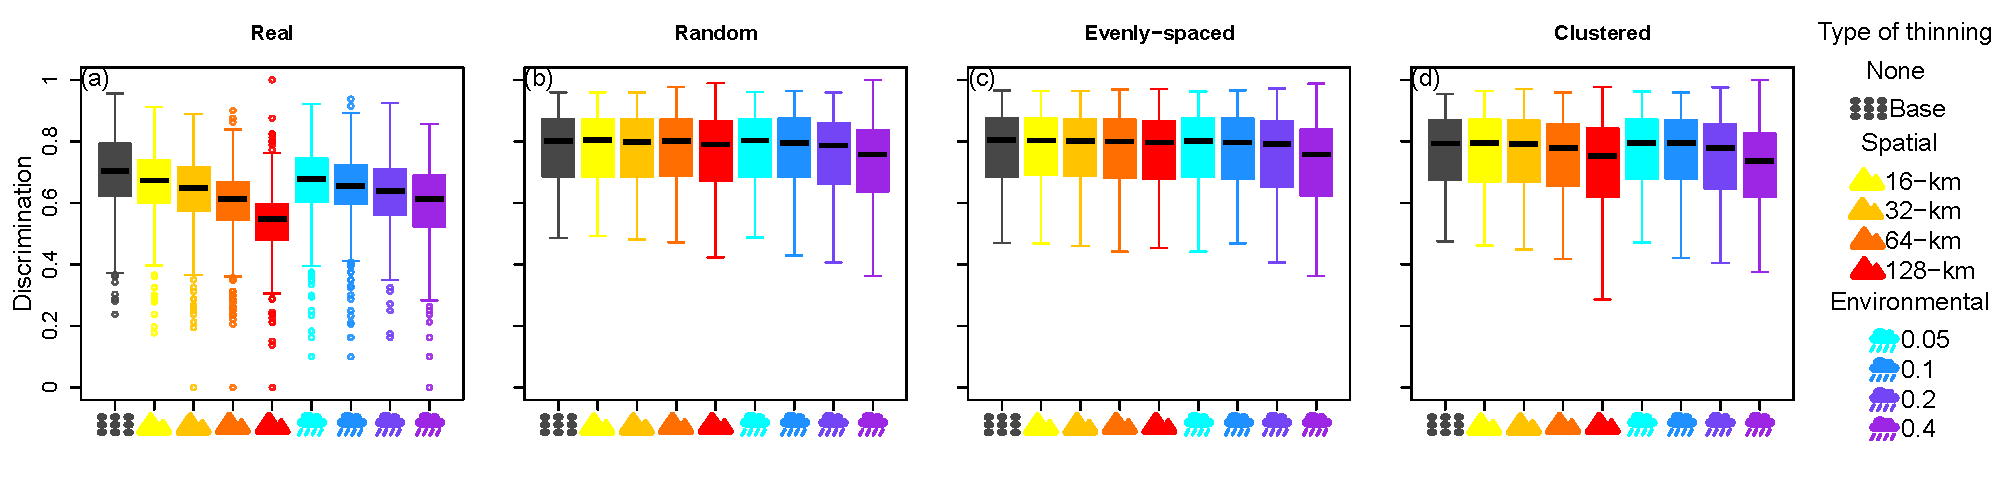
\includegraphics[width=1\textwidth]{Plots/FigureS11}} 
\caption[Effects of thinning on GLM discrimination]{The effects of spatial and environmental thinning on GLM discrimination (AUC) of real species (a), and virtual species with random (b), clustered (c), and evenly-spaced (d) sampled occurrence points.}
 \label{fig:S11}
\end{figure}
\clearpage
\begin{figure}[h!]
\centering
%\graphicspath{ {c:/Teste/Chapter-1-Protocol/Manuscript/Plots/}  }
\centerline{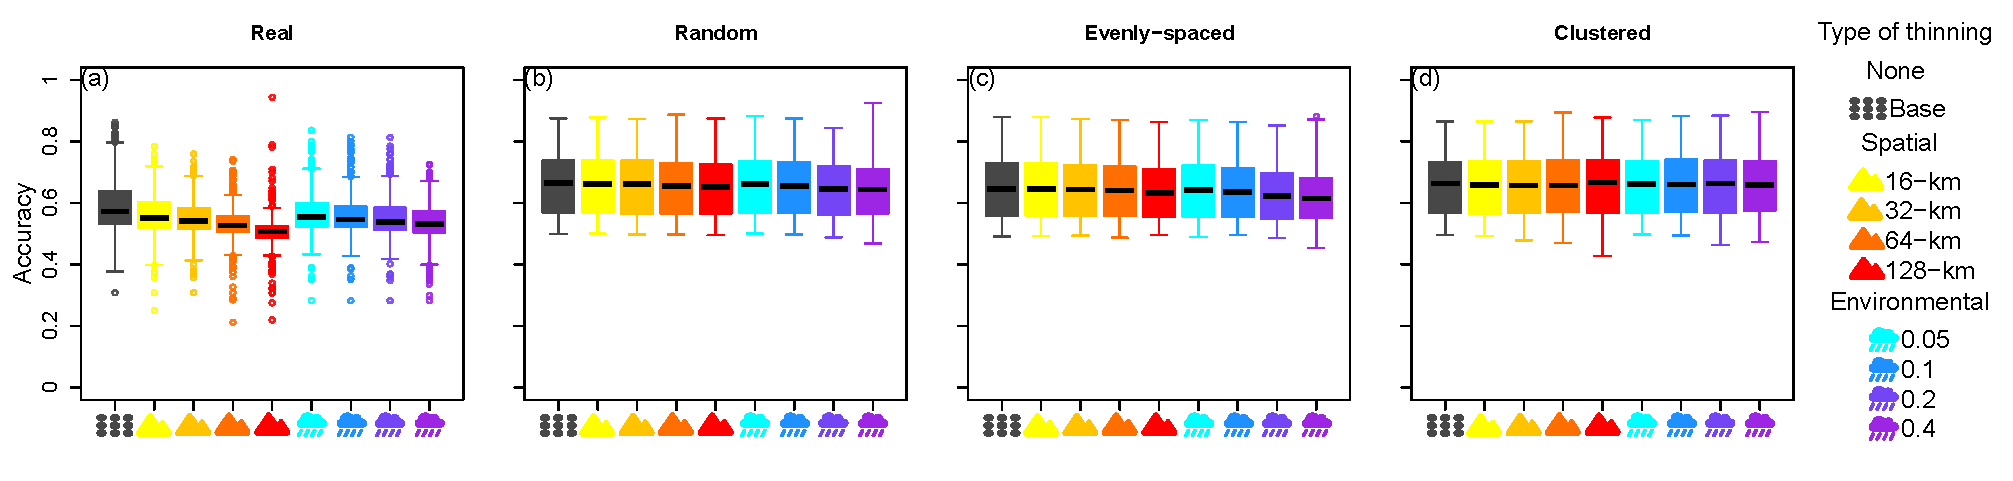
\includegraphics[width=1\textwidth]{Plots/FigureS12}} 
\caption[Effects of thinning on GLM accuracy]{The effects of spatial and environmental thinning on GLM accuracy of real species (a), and virtual species with random (b), clustered (c), and evenly-spaced (d) sampled occurrence points.}
 \label{fig:S12}
\end{figure}

\begin{figure}[h!]
\centering
%\graphicspath{ {c:/Teste/Chapter-1-Protocol/Manuscript/Plots/}  }
\centerline{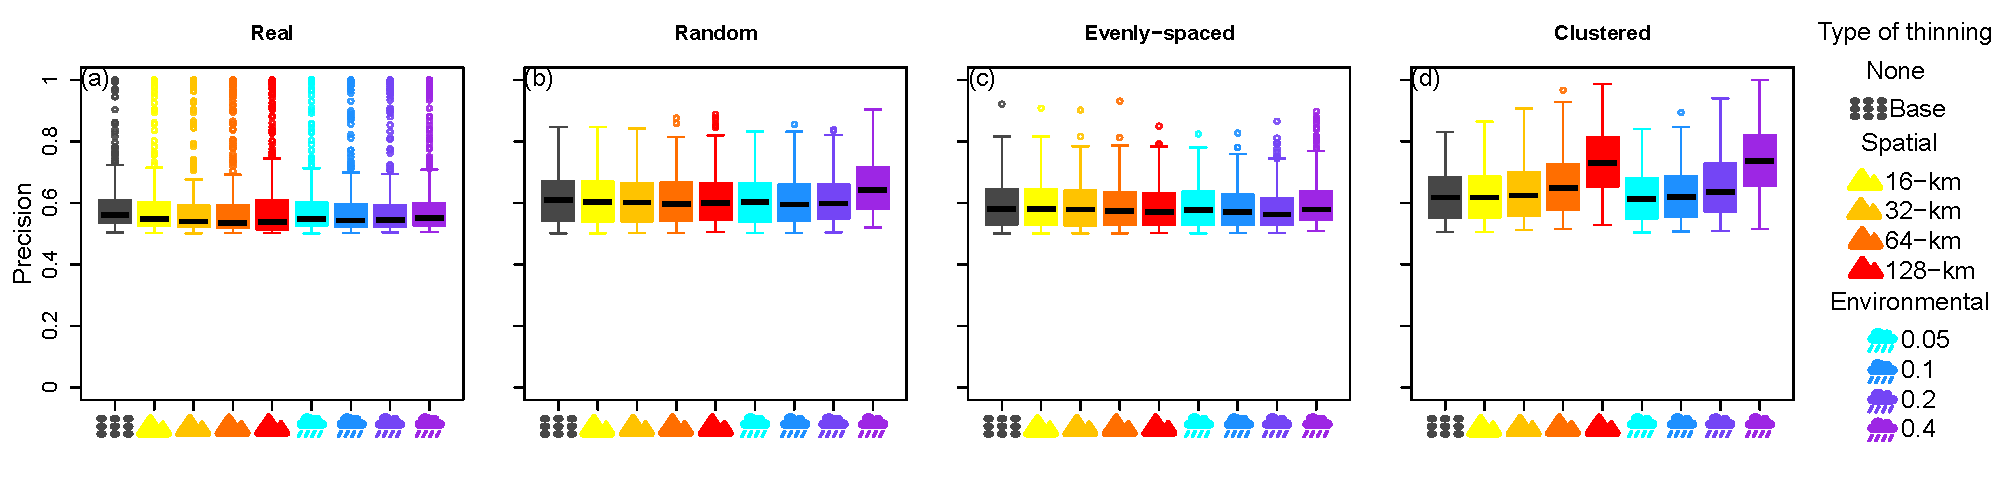
\includegraphics[width=1\textwidth]{Plots/FigureS13}} 
\caption[Effects of thinning on GLM precision]{The effects of spatial and environmental thinning on GLM precision of real species (a), and virtual species with random (b), clustered (c), and evenly-spaced (d) sampled occurrence points.}
 \label{fig:S13}
\end{figure}

\begin{figure}[h!]
\centering
%\graphicspath{ {c:/Teste/Chapter-1-Protocol/Manuscript/Plots/}  }
\centerline{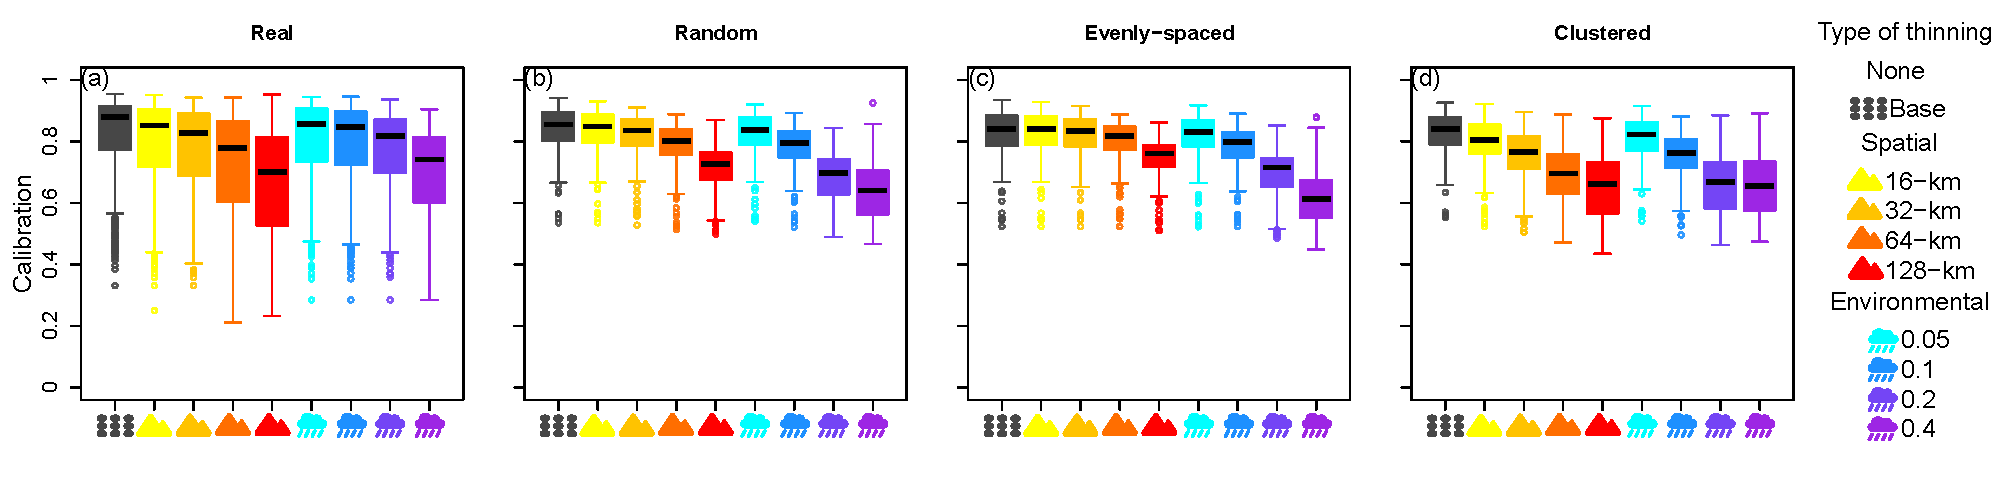
\includegraphics[width=1\textwidth]{Plots/FigureS14}} 
\caption[Effects of thinning on GLM calibration]{The effects of spatial and environmental thinning on GLM calibration of real species (a), and virtual species with random (b), clustered (c), and evenly-spaced (d) sampled occurrence points.}
 \label{fig:S14}
\end{figure}
 
\subsection*{\textbf{Using GAM}}

Thinning occurrence points affected GAM performance similarly to MaxEnt. Spatial and environmental thinning smilarly decreased discrimination, accuracy and calibration of GAM for real species (Figure \ref{fig:S15}a, \ref{fig:S16}a, \ref{fig:S18}a) and virtual (Figure \ref{fig:S15}b-d, \ref{fig:S16}b-d, \ref{fig:S18}b-d) species. In these cases, environmental thinning had a stronger negative effect on GAM discrimination, accuracy and calibration of virtual species with random and evenly-spaced occurrence points whereas both environmental and spatial thinning had equally strong negative effects on GAM discrimination, accuracy and calibration of virtual species with clustered occurrence points. In contrast, spatial and environmental thinning increased GAM precision for real (Figure \ref{fig:S17}a) and virtual (Figure \ref{fig:S17}b-d) species especially when larger thinning distances were used, although this result has no significance given that model accuracy decreased when thinning was used. Overall, our results show that spatial and environmental thinning had consistent negative effects on GAM performance, and that these negative effects tended to be stronger when larger thinning distances were used.




\begin{figure}[h!]
\centering
%\graphicspath{ {c:/Teste/Chapter-1-Protocol/Manuscript/Plots/}  }
\centerline{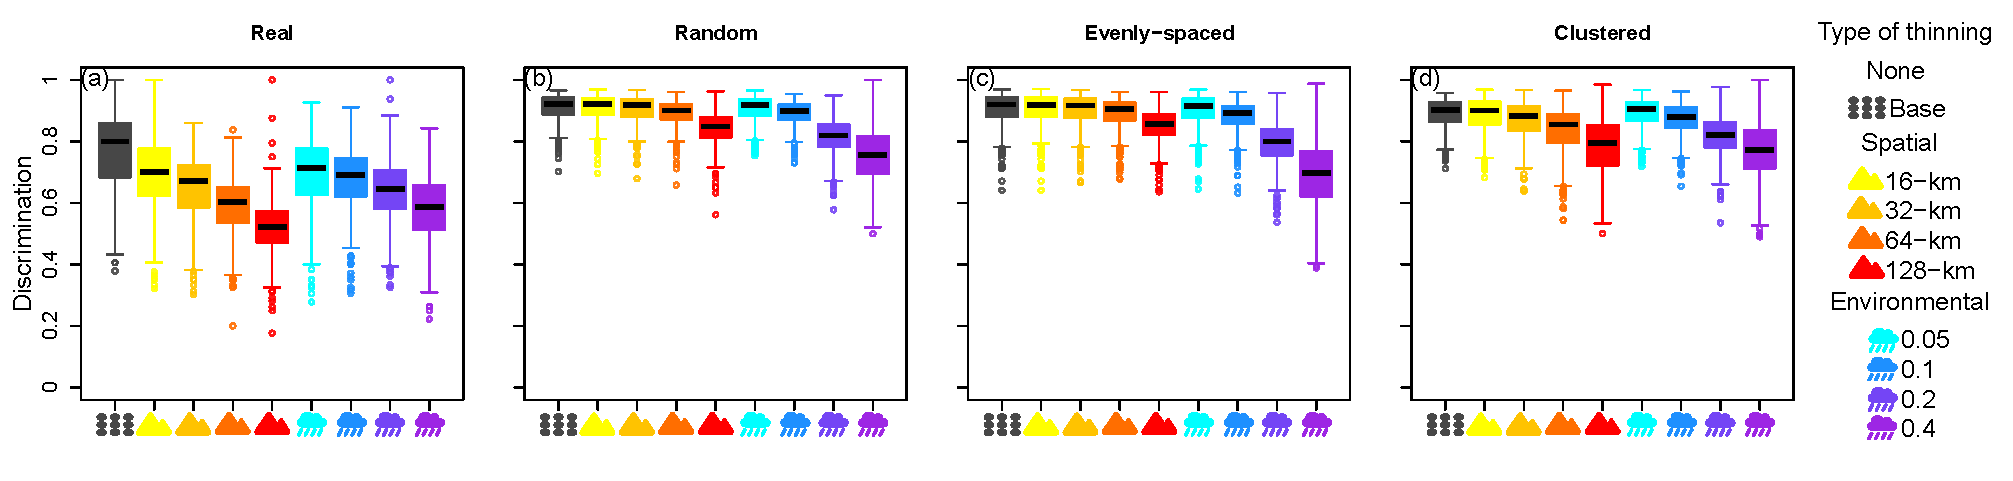
\includegraphics[width=1\textwidth]{Plots/FigureS15}} 
\caption[Effects of thinning on GAM discrimination]{The effects of spatial and environmental thinning on GAM discrimination (AUC) of real species (a), and virtual species with random (b), clustered (c), and evenly-spaced (d) sampled occurrence points.}
 \label{fig:S15}
\end{figure}

\begin{figure}[h!]
\centering
%\graphicspath{ {c:/Teste/Chapter-1-Protocol/Manuscript/Plots/}  }
\centerline{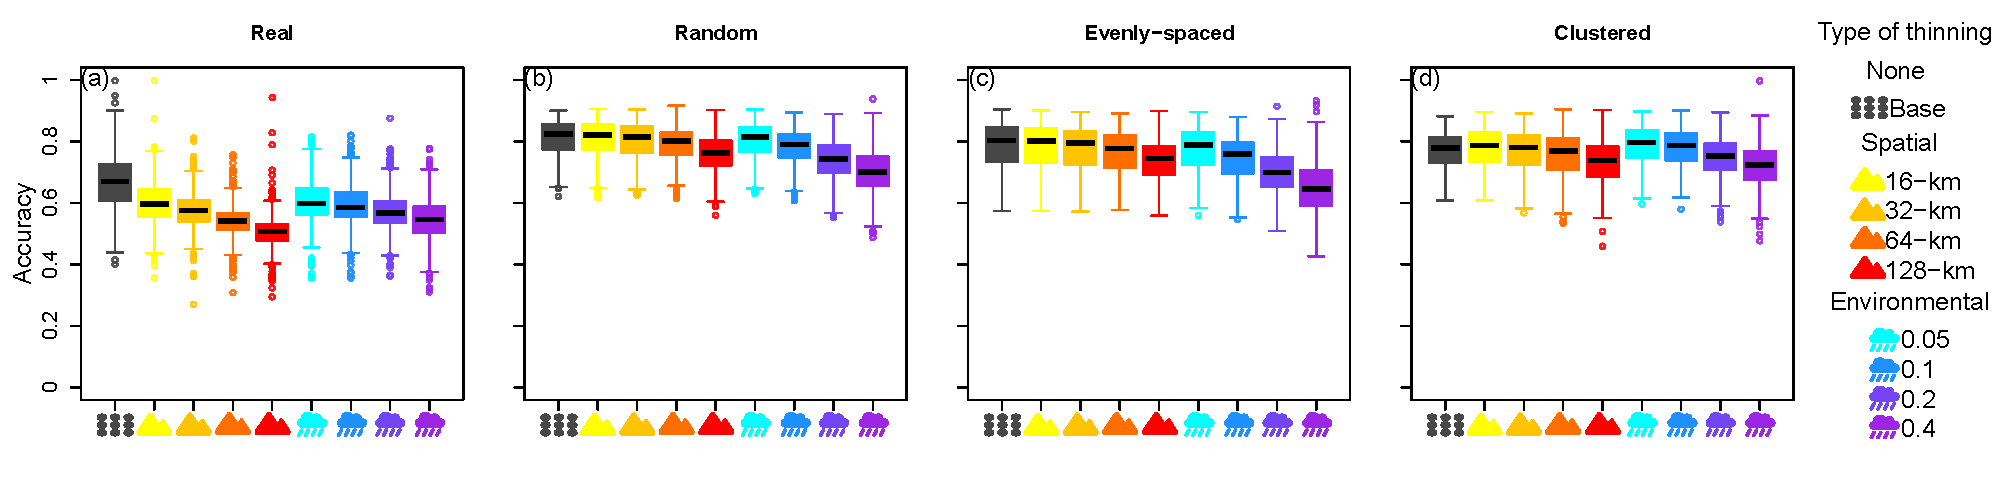
\includegraphics[width=1\textwidth]{Plots/FigureS16}} 
\caption[Effects of thinning on GAM accuracy]{The effects of spatial and environmental thinning on GAM accuracy of real species (a), and virtual species with random (b), clustered (c), and evenly-spaced (d) sampled occurrence points.}
 \label{fig:S16}
\end{figure}

\clearpage
\begin{figure}[h!]
\centering
%\graphicspath{ {c:/Teste/Chapter-1-Protocol/Manuscript/Plots/}  }
\centerline{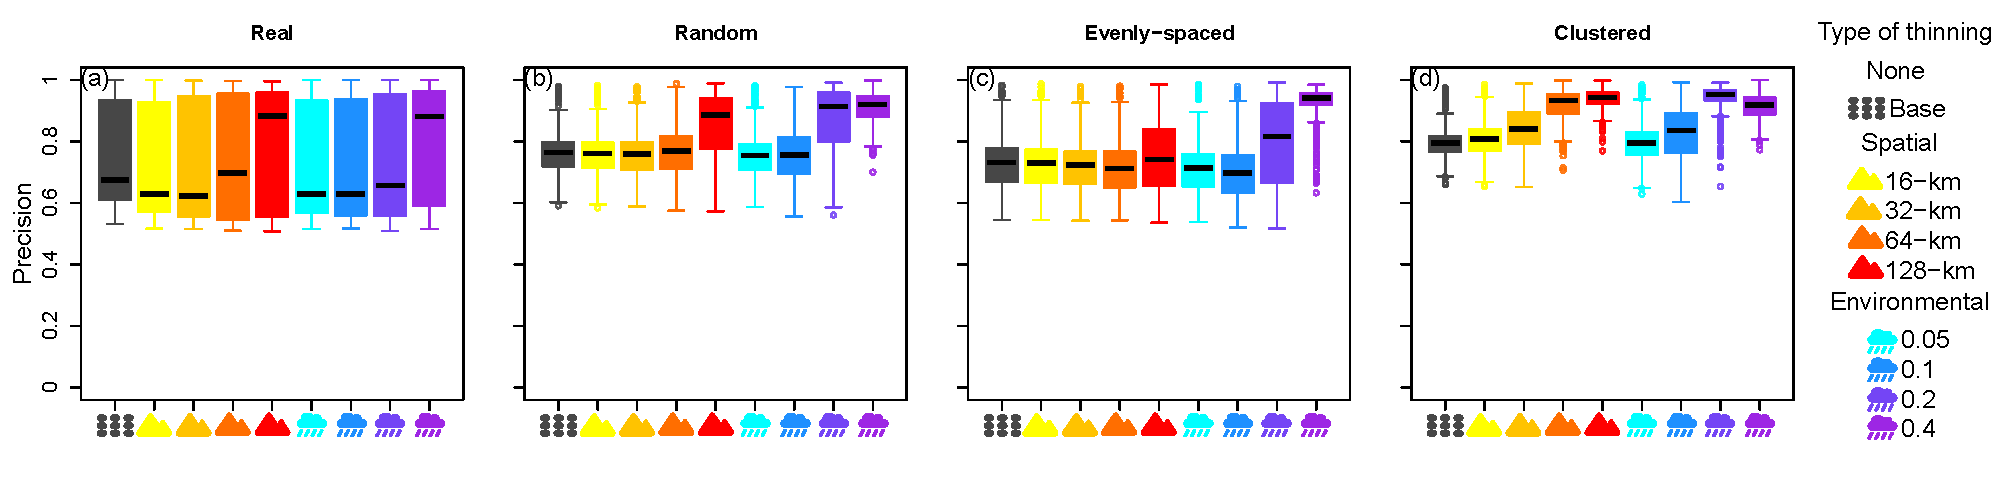
\includegraphics[width=1\textwidth]{Plots/FigureS17}} 
\caption[Effects of thinning on GAM precision]{The effects of spatial and environmental thinning on GAM precision of real species (a), and virtual species with random (b), clustered (c), and evenly-spaced (d) sampled occurrence points.}
 \label{fig:S17}
\end{figure}

\begin{figure}[h!]
\centering
%\graphicspath{ {c:/Teste/Chapter-1-Protocol/Manuscript/Plots/}  }
\centerline{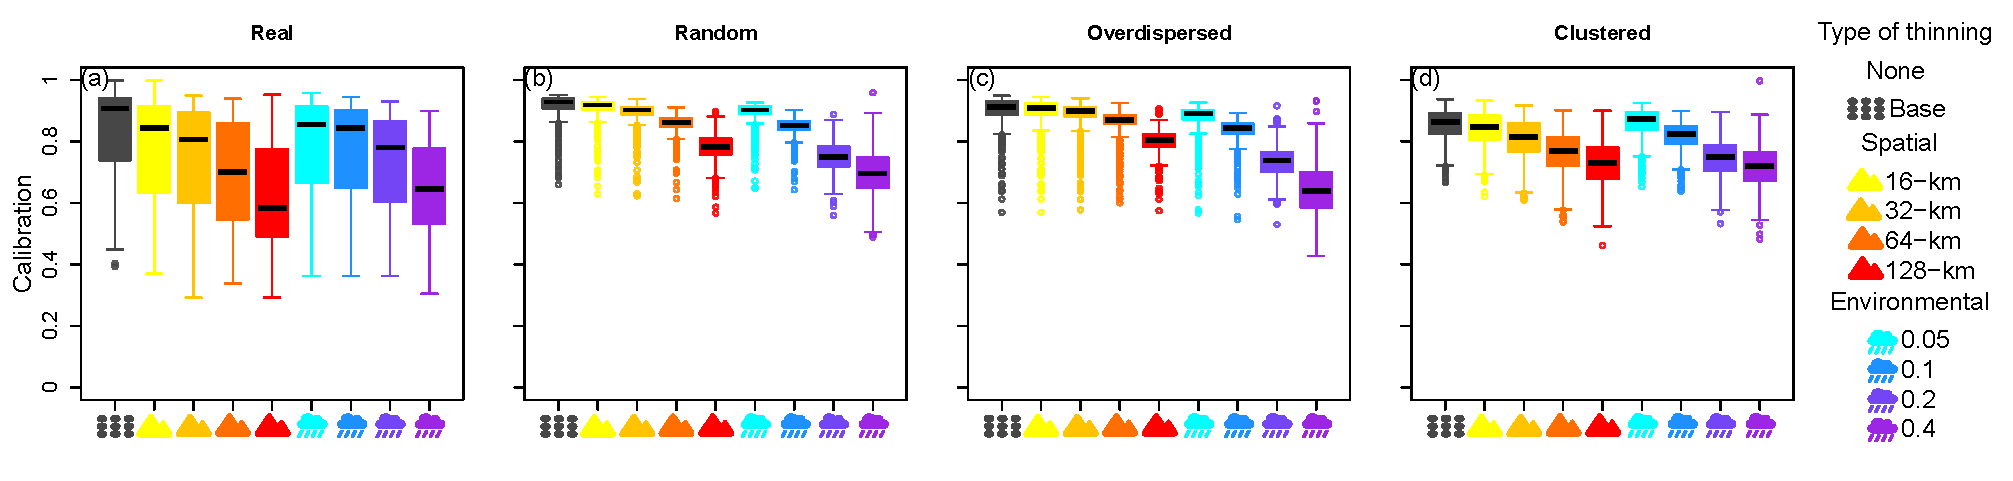
\includegraphics[width=1\textwidth]{Plots/FigureS18}} 
\caption[Effects of thinning on GAM calibration]{The effects of spatial and environmental thinning on GAM calibration of real species (a), and virtual species with random (b), clustered (c), and evenly-spaced (d) sampled occurrence points.}
 \label{fig:S18}
\end{figure}


